\section{Proxy Re-Encryption}

\subsection{Introduction to Proxy Re-Encryption}

\blockquote{In a proxy re-encryption scheme a semi-trusted proxy converts a ciphertext for Alice into a ciphertext for Bob without seeing the underlying plaintext}\autocite{greenateniese:2006:article}

Fundamentally, proxy re-encryption is the process of taking a message $M_a$, encrypted by a party $P_a$, and re-encrypting it to be passed to party $P_b$. The message is then represented by $M_b$, such that it is only readable by party $P_b$. Through the re-encryption process, the message is never actually decrypted, such that the data is never revealed to any non-trusted parties (including the proxy itself). This process relies on the functional relationship between the two ciphertexts, with the characteristics of the proxy re-encryption processed determined by the topology of this function.



\begin{figure}[H]
  \centering
  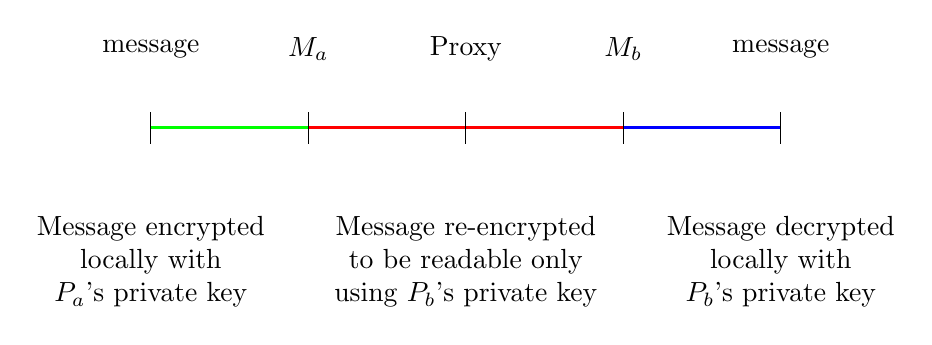
\begin{tikzpicture}

  \node at (0, 1)   {message} ;
  \node at (2, 1)   {$M_a$}   ;
  \node at (4, 1)   {Proxy}   ;
  \node at (6, 1)   {$M_b$}   ;
  \node at (8, 1)   {message} ;

  \draw [very thick, green] (0,0)   -- (2,0)   ;
  \draw [very thick, red]   (2,0)   -- (6,0)   ;
  \draw [very thick, blue]  (6,0)   -- (8,0)   ;
  \draw                     (0,-.2) -- (0, .2) ;
  \draw                     (2,-.2) -- (2, .2) ;
  \draw                     (4,-.2) -- (4, .2) ;
  \draw                     (6,-.2) -- (6, .2) ;
  \draw                     (8,-.2) -- (8, .2) ;

  \node[align=center, below] at (0, -1)%
    {Message encrypted\\locally with\\$P_a$'s private key};
  \node[align=center, below] at (4, -1)%
    {Message re-encrypted\\to be readable only\\using $P_b$'s private key};
  \node[align=center, below] at (8, -1)%
    {Message decrypted\\locally with\\$P_b$'s private key};

  \end{tikzpicture}
  \caption{
    Journey of a message using a proxy re-encryption scheme.
  }
  % \label{fig:pre_example}
\end{figure}


There are many different ways to implement proxy re-encryption, with differing level of ease, complexity, and, most importantly, security. One must consider whether a unidirectional scheme or a bidirectional scheme is preferred. One must also consider that a proxy is, by definition of re-encryption without exposing the underlying data, a semi-trusted entity; we allow the proxy to manipulate the encrypted data we pass to it, without full control of seeing or sharing the data further than we wish.

\subsection{Applying Proxy Re-Encryption}



\subsection{ZeroDB}
